%%%%%%%%%%%%%%%%%%%%%%%%%%%%%%%%%%%%%%%%%%%%%%%%%%%
%% P3: Phenomenology of Particle Physics                         
%%
%% Author:  André Rubbia                   		 
%%
%% Figure 20.11 Non-relativistic potential $V_{q\bar q}(r)$ between the quark and antiquark in the quarkonium system.
%%
%% This work is licensed under the Creative Commons Attribution 4.0 International License. 
%% To view a copy of this license, visit http://creativecommons.org/licenses/by/4.0/ or 
%% send a letter to Creative Commons, PO Box 1866, Mountain View, CA 94042, USA.
%%
%%%%%%%%%%%%%%%%%%%%%%%%%%%%%%%%%%%%%%%%%%%%%%%%%%%

\documentclass[a4paper,10pt]{article}

\usepackage[T1]{fontenc}
\usepackage[utf8]{inputenc}
\usepackage{lmodern}
\usepackage[labelfont=bf]{caption}
\usepackage{upgreek}

\usepackage{tikz}
\usepackage{pgfplots}
\pgfplotsset{compat=1.17}
\usepgfplotslibrary{ternary}
\usepgfplotslibrary{fillbetween}
\usepgfplotslibrary{external}

\def\d{\mathrm{d}}

\begin{document}

%%%%%%%%%%%%%%%%   FIGURE  %%%%%%%%%%%%%%%%%%%%%%%%%%%%%%
\begin{figure}[htb]
\centering
\pgfplotsset{every axis/.append
    style={
%    font=\large,
    width=0.9*\textwidth,
    height=0.9*\textwidth,
    line width=1pt,
    tick style={line width=0.8pt}}}
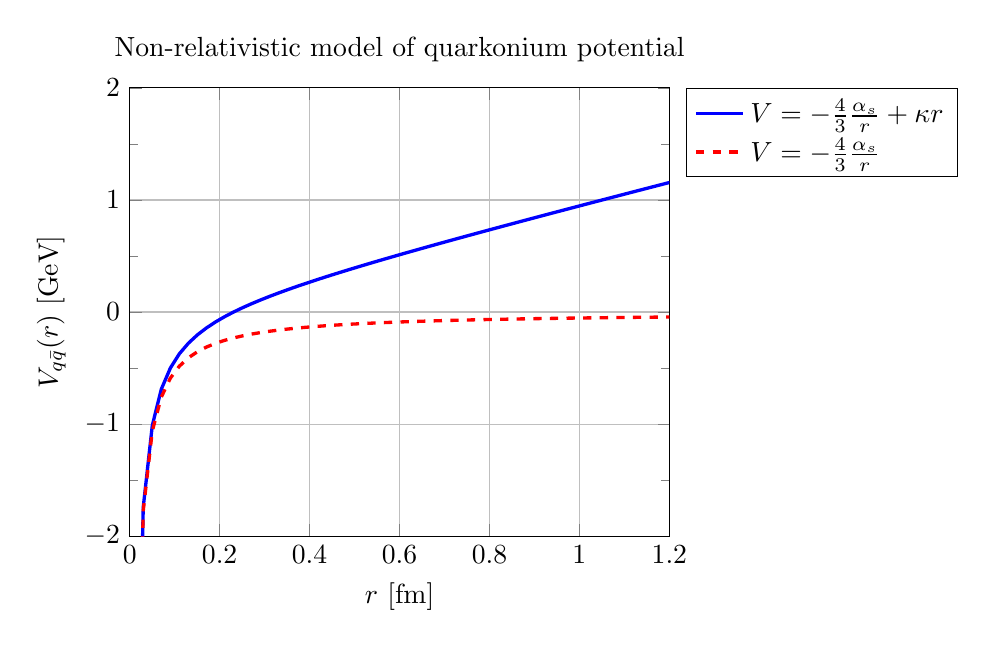
\begin{tikzpicture}[scale=1.]
    \begin{axis}[
        title=Non-relativistic model of quarkonium potential,
        xlabel={$r$ [fm]},
        ylabel={$V_{q\bar q}(r)$ [GeV]},
        xmin=0, xmax=1.2,
        ymin = -2, ymax=2,
        minor y tick num=1,
        grid = major,
        legend entries={
        $V=-\frac{4}{3}\frac{\alpha_s}{r}+\kappa r$,
        $V=-\frac{4}{3}\frac{\alpha_s}{r}$,
        },
        legend style={legend pos = outer north east},
	legend cell align = {left}
    ]
%  -(4/3)*alphas*0.2/x+kappa*x
% alphas=0.2, kappa=1
        \addplot [blue,very thick,domain=0.01:2, samples=100] {-(4./3.)*0.2*0.2/x+1.0*x};
% alphas=0.2, kappa=0
        \addplot [red,very thick,dashed,samples=100,domain=0.01:2] {-(4./3.)*0.2*0.2/x};
  \end{axis}
\end{tikzpicture}%
\caption{Non-relativistic potential $V_{q\bar q}(r)$ between the quark and antiquark in the quarkonium system for
$\alpha_S=0.2$ and $\kappa=1$~GeV/fm.}
\end{figure}
%
%%%%%%%%%%%%%%%%   END FIGURE  %%%%%%%%%%%%%%%%%%%%%%%%%%%%%%
%
\end{document}
